
\chapter{A New Generation of Knowledge Graph Construction Engines}
\label{chapter:mappig-translation}

\epigraph{The primary goal of a researcher should be to continually challenge science with creative ideas}{\textit{Oscar Corcho}}


Database technologies play a vital role in the development of information systems for all sorts of organizations. So far, relational databases (RDB) are still the dominating type of structure and technology used for data management inside organizations, although other formats (e.g. JSON, spreadsheets, XML) and types of databases (e.g. noSQL, graph databases) have also emerged as alternatives for data representation and management in the last decades. 

\begin{figure*}[!ht]
    \centering
    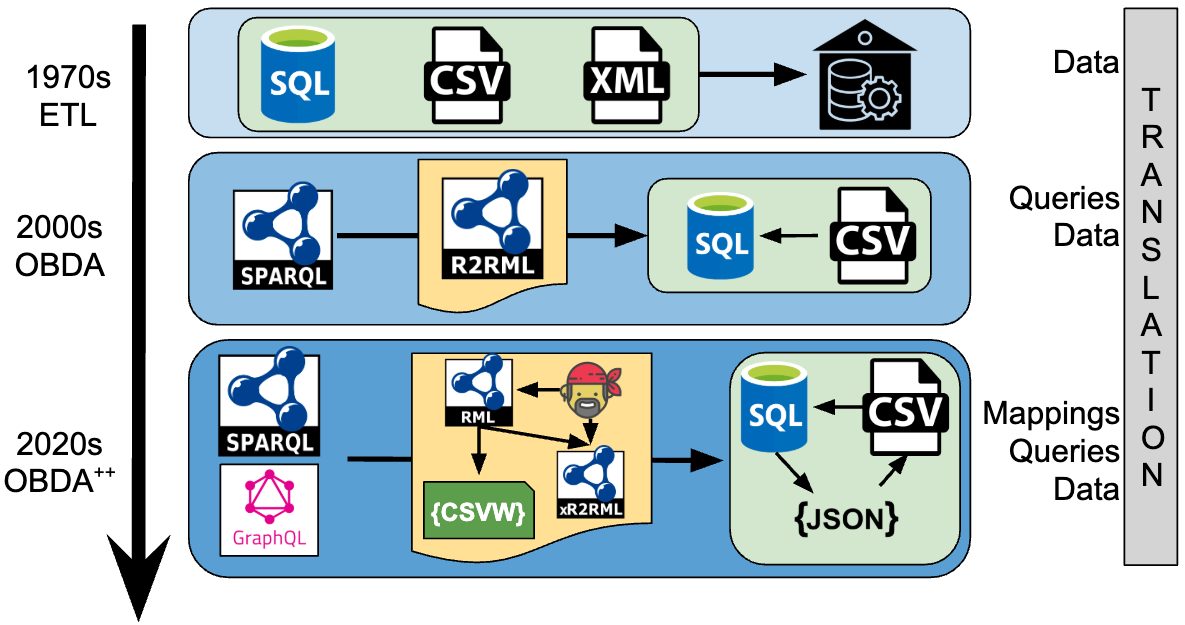
\includegraphics[width=1\columnwidth]{./figures/mt_obda_timeline.png}
    \caption[Timeline of data integration techniques]{\textbf{Timeline of data integration techniques}. During the 1970s ETL approaches started with data translation techniques, current generation of KGC incorporated techniques for query translation and next generation of KGC systems which mapping translation approaches are to be applied.
    }
    \label{fig:obdatimeline}
\end{figure*}

In the early days of information system development, it was natural for organizations to develop their own data models, which were strongly aligned with their activities. This led to a large heterogeneity of data models across organizations, and even across different departments inside the same organization. Such heterogeneity was especially evident in the case of organizational changes, merges, etc. These situations made researchers and professionals start working on solutions for data integration, where data from several sources needed to be accessible according to a unified and global view over such local heterogeneous data sources. Data warehouses were used in order to align and materialize data from different sources, normally from the same organization, so as to provide support for analytical queries and for the generation of reports. Popular technologies used in production systems worldwide included the use of Extract-Transform-Load (ETL) workflows to overcome heterogeneity and ensure the availability of data in such data warehouses or on integrated databases. Indeed, these approaches are still strongly used nowadays.

In the meantime, data integration challenges became even more relevant when organizations started using Web technologies to provide access to their data (via Web Services, REST APIs or using Semantic Web and Linked Data approaches), both for their own information system development as well as for data sharing, and later on when public administrations started publishing open data according to  public-sector information reuse initiatives. Availability and heterogeneity of data (both in terms of content and format) is nowadays present at an unprecedented level. Following the aforementioned ETL approaches, the term data lake has been rather recently coined to refer to an evolution of data warehouses that considers not only structured data but also the other types of (semi-)structured and unstructured formats in which data is made available nowadays, as discussed above.

Over these decades, several approaches have been proposed to tackle data integration challenges. We are specially interested in those that fall under the area of Ontology Based Data Access (OBDA) and Integration (OBDI)~\citep{poggi2008linking}, which is recently also defined as Knowledge Graph Construction (KGC) methods. From now on we will refer to all of them, in a general manner, as KGC. As we have already mentioned in Chapter \ref{chap:intro} and Chapter \ref{chap:soa}, in KGC, ontologies are used as a global view over heterogeneous data sources and mappings are used to describe such relationships in a declarative manner. Many different types of KGC mapping languages have been proposed over the last decades, with a large variety of syntax and formats especially in the early ones. Since the standardization of languages like RDF and OWL, several languages were proposed focused on the transformation from relational databases into RDF (e.g. D2R~\citep{bizer2004d2rq}, R2O~\citep{barrasa2004r2o}). This led to the creation of the RDB2RDF W3C Working Group, which published two recommendations for transforming the content of relational databases into RDF: Direct Mapping \citep{arenas2013direct} and R2RML \citep{R2RML}.

As we describe in Chapter \ref{chap:soa}, a bit after R2RML was recommended, and because of its use in different types of contexts, new needs and requirements arose, especially in relation to supporting other formats beyond relational databases, and this resulted in the creation of many new mapping languages, such as RML \citep{dimou2014rml} (to deal with CSVs, JSON and XML data sources), xR2RML \citep{michel2015translation} (to deal with MongoDB), KR2RML \citep{slepicka2015kr2rml} (to deal with nested data), CSVW\footnote{\url{https://www.w3.org/ns/csvw}} (to describe CSV files on the Web), or D2RML \citep{chortaras2018d2rml} (for XML, JSON and REST/SPARQL endpoints). In addition to declarative languages, non-declarative mapping languages have also been proposed, such as SPARQL-Generate \citep{lefranccois2017sparql}, Helio\footnote{\url{https://helio.linkeddata.es/}},  TARQL\footnote{\url{https://github.com/tarql/tarql}} or Triplify~\citep{auer2009triplify}.

\noindent\paragraph{\textbf{Why so many mapping languages?}}
There are several reasons why new mapping languages are needed. The first and main reason is that a typical mapping language is designed to work with a specific \textbf{data format} (e.g. R2RML is focused on relational databases). Even for a more generic-purpose mapping language, such as RML, there may still be a need to extend it to support a more specific technology, such as nested data hierarchies. Another reason is \textbf{readability and compactness}. Most mapping languages are designed in a format to be parsed by machines and they do not take into account human readability. Examples of languages created to account for this are R2RML-Iterator (for statistical CSV files) \citep{chaves2018virtual} or YARRRML \citep{Heyvaert2018Declarative}. Lastly, many of existing mapping languages \textbf{lack formalization}, making it difficult to apply, for example, query translation techniques. 

Therefore, the current situation of a KG construction practitioner that needs to provide access to a varied set of heterogeneous data sources is that there are many different options to select from, and it is difficult to determine which one is better for each situation. Languages are not necessarily interoperable, and many of them come associated with a very specific engine that supports them. At the same time, it is clear that most of these languages share many common aspects, such as the description of where the data comes from, how IRIs can be created for resources, how triples need to be generated (in a materialized or virtual way), etc. Having the possibility of translating among these different languages, covering at least those common characteristics that are shared across languages, would allow practitioners to have the possibility of selecting a wider set of engines to implement their KG construction system, or the different parts of a KG.

In this chapter, we lay out our vision that the next generation of KGC systems should take advantage of this proliferation of mapping languages. In other words, in addition to the data translation and query translation techniques that have been widely addressed in the state of the art of KGC so far, the KGC research community will need to think carefully about how to address mapping translation (See Figure \ref{fig:obdatimeline}), as we describe in the next sections.


\section{Mapping Translation: Concept Definition}
We define the mapping translation concept as a function that transforms a set of mappings described in one language (we call them original mappings) into a set of mappings described in another language (we call them target mappings). 

Our next step is to attach desirable properties for such a function. In this line, we propose to use and adapt some properties that have been described by \citep{sequeda2012directly} and \citep{hartig2017foundations} in their works. To be more specific, those properties are \textit{information preservation} and \textit{query result preservation} (Figure \ref{fig:mt}).

The \textbf{Information Preservation Property (IPP)} applied to a mapping translation function states that at least there is a function so that its application over the information generated by the application of the target mappings over the original data source returns the same information generated by the application of the original mappings over the same data source.

The \textbf{Query Result Preservation Property (QRPP)} applied to a mapping translation function states that for any query that can be evaluated over the information generated from the application of the original mappings to the original data source, there is at least a function to generate another query that can be evaluated over the information generated by the application of the target mappings to the same data source, in such a way that both queries return the same results.


Finally, using these two properties, we define the concepts of weak and strong semantics preservation for a mapping translation function, as follows: a mapping translation function exhibits \textbf{weak semantics preservation} if only IPP holds. If both IPP and QRPP are satisfied, then we say that it holds the \textbf{strong semantics preservation} property.


\begin{figure}[!t]
    \centering
    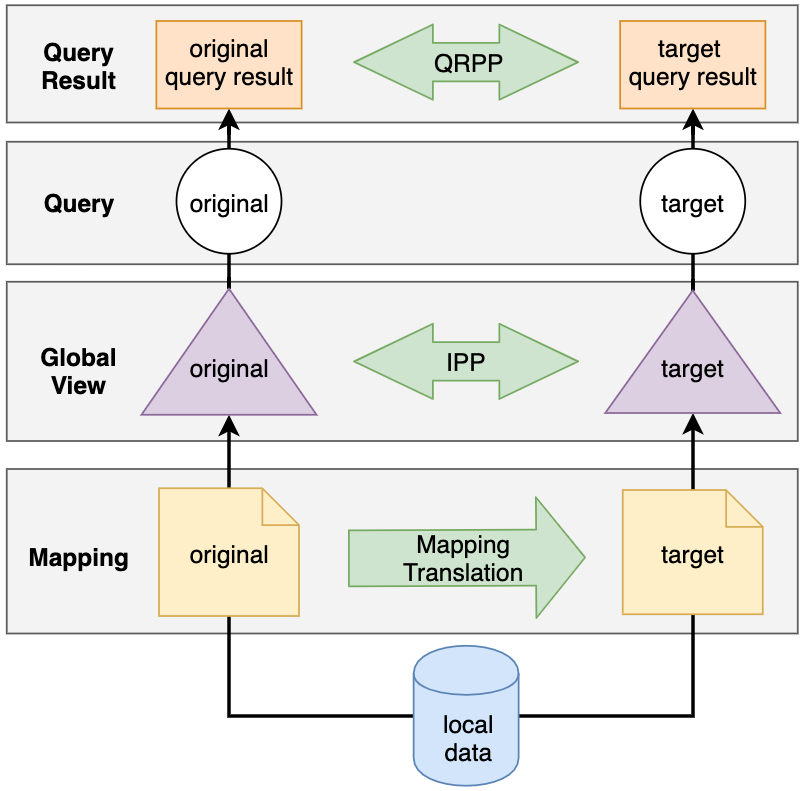
\includegraphics[width=0.6\columnwidth]{./figures/mapping-translator.png}
    \caption[Mapping translator properties]{\textbf{Mapping Translator Properties.} The results (triangles) may satisfy the IPP property after the application of the source and target mappings over the same data. In the same way, query results (rectangles) may satisfy the QRPP property when equivalent queries are evaluated over the source and target results.}
    \label{fig:mt}
\end{figure}


\section{Mapping Translation by example}
In this section we identify a set of scenarios and challenges in the creation and use of KGC mapping languages, where mapping translation is relevant. We describe the challenge and provide some references to some of the work presented in the literature addressing or acknowledging it. The presented use cases are summarized in Table \ref{tab:chap4_summary}.

\begin{table}[!ht]
\centering
\caption{Summary of Mapping Translation Approaches}
\label{tab:chap4_summary}
\resizebox{0.65\textwidth}{!}{%
\begin{tabular}{c|c|c}
\hline
\textbf{Use Case}         & \textbf{Engine} & \textbf{Translation}     \\ \hline
Maintenance               & Mapeathor       & Excel-to-[R2]RML           \\ \hline
Maintenance               & yarrrml-parser  & YARRRML-to-RML           \\ \hline
Maintenance               & r2rml-statistic & R2MLIterator-to-R2RML    \\ \hline
Maintenance               & ShExML          & ShExML-to-RML            \\ \hline
Declarative to Programmed & morph-graphQL   & R2RML-to-GraphQLResolver \\ \hline
Access                    & Morph-CSV       & RML(+FnO)-to-R2RML       \\ \hline
Optimizations                    & FunMap          & RML(+FnO)-to-RML          \\ \hline
Optimizations/Semantics   & ontop           & R2RML-to-OBDA            \\ \hline
\end{tabular}%
}
\end{table}



\subsection{Improving mapping creation and maintenance}

Creating and maintaining KGC mappings is usually difficult, since mapping languages have been created so that they can be consumed by the corresponding engines, and they commonly suffer from readability and compactness problems. With respect to \textbf{readability}, several approaches have focused on providing mapping editors (e.g. \citep{heyvaert2016rmleditor,iglesias2020mapeathor}) so that mappings are easier to create by non experts. However, these editors are usually limited to some features of the mapping language or to a specific version of the mapping language specification, and in general they still require knowledge about the underlying mapping language syntax. With respect to \textbf{compactness}, there are cases where the generated mapping documents are very long and repetitive, making it difficult to create and maintain~\citep{chaves2018virtual}. For instance, this is the case when a KGC approach is used to provide access to multidimensional data sources, such as the ones commonly used to publish statistical data. We describe three cases where mapping translation ideas are already being applied to address these issues. 

YARRRML~\citep{Heyvaert2018Declarative} is a serialisation of RML mappings that uses the YAML (a human-readable data serialization language) format\footnote{\url{https://yaml.org/}}. It is designed with the objective to reduce the size and verbosity of RML. There is no specific engine or parser to exploit YARRRML mappings in an KGC setting. Instead, the tool Matey\footnote{http://rml.io/yarrrml/matey/} is in charge of translating YARRRML mappings into RML, so that any RML-compliant OBDA engine can be used to exploit them. ShExML~\citep{garcia2020shexml} presents a similar work, where the authors extend the syntax of ShEx shapes constraints~\citep{prud2014shape} to support the construction of KGs from heterogeneous data sources. They conduct a user evaluation and observe that their approach is easy to use and maintain. To exploit all the benefits from the RML engines, they provide a translator engine from ShExML to RML.

In the case of multidimensional data (e.g. official statistics data), the W3C RDF DataCube recommendation is the ontology that is commonly used as a global view in an KGC setting. In most cases, the amount of mappings that would need to be created to link the original data source with the ontology will be rather large and with similar structure. Therefore, there is a high risk that the [R2]RML mapping document(s) generated in the end will contain clerical errors due to copy\&paste\&edit operations. Furthermore, they will be difficult to maintain. As a result, R2RML-Iterator~\citep{chaves2018virtual} is proposed as a simplified mapping language specifically designed for this type of data. The proposal is detailed in Section \ref{sec:chap4_rmlc}.


\subsection{From declarative mappings to programmed adapters}
Introduced in 2000, REST \citep{fielding2000architectural} has become now the most popular architecture for the provision of web services and the implementation of Web-based applications. However, the complexity of software development continues evolving, and aspects that received little attention, such as the size of data being exchanged/transmitted or the number of API calls being made, are now becoming more relevant in the context of mobile application development. As a result, problems like \textit{over-fetching} (a REST endpoint returns more data than what is required by the client) and \textit{under-fetching} (a single REST endpoint does not provide sufficient information requested by the client) are now being discussed. In order to address these problems, Facebook proposed the GraphQL query language \citep{graphql}, used internally since 2012 and released for public use in 2015. Since then it has been increasingly adopted, and GraphQL is now supported by multiple GraphQL engines for major programming languages (e.g. JavaScript, Python, Java, Golang, Ruby).

The two main components of a GraphQL server are the \textbf{schema} and the \textbf{resolvers}. The GraphQL schema specifies the type of an object together with the fields that can be queried. GraphQL resolvers are data extraction functions implemented in a programming language that are responsible to translate GraphQL queries into queries supported by the underlying datasets (e.g. GraphQL to SQL). In addition, query planning tools have been developed in order to translate GraphQL queries into other query languages (e.g. dataloader\footnote{\url{https://github.com/facebook/dataloader}}, joinmonster\footnote{\url{https://join-monster.readthedocs.io/en/latest/}}).

In a recent paper~\citep{priyatna2019morph} we proposed the use of the mapping translation concept to facilitate the generation of GraphQL resolvers. We propose specifying mappings in R2RML, which is a well-defined and formalized mapping language, and apply a mapping translation technique to generate automatically the corresponding GraphQL schemes and resolvers in different programming languages. Our intuition is that following this approach, GraphQL resolver will be easier to maintain, as they are declarative and independent from any programming language. The details of this approach are presented in Section \ref{chap6_morphgraphql}.

\subsection{Providing access to semi-structured data}
Semi-structured data formats are one of the most widely used formats to publish data on the Web. Although existing mapping languages provide support for this type of data sources, existing engines are mostly focused on the generation (materialization) of RDF-based knowledge graphs, with only a few proposals (e.g. xR2RML~\citep{michel2015translation}) focused on the application of query-translation techniques (virtualization) over such types of data sources.

In the specific case of spreadsheets (CSV), providing access to this format is difficult for two main reasons: (i) CSV does not provide its own query language, (ii) there are some transformations that are commonly needed when treating data available in CSVs. For solving the first issue, query translation techniques have been applied over such data format by considering a CSV file as a single table that can be loaded in an RDB. For the second issue, some extensions of well-known mapping languages (RML together with the Function Ontology~\citep{de2017declarative}) and annotations following the CSVW specification~\citep{tennison2015model} can be used.

Morph-CSV applies the concept of mapping translation for enhancing OBDA query translation over CSV files from SPARQL. It exploits the information of CSVW annotations and RML+FnO mappings to create an enriched RDB representation of the CSV files together with the corresponding R2RML mappings, allowing the use of existing query translation (SPARQL-to-SQL) techniques implemented in R2RML-compliant OBDA engines. This contribution is detailed in Section \ref{chap6_morphgcsv}.


\subsection{Understanding the semantics of mapping languages}
To the best of our knowledge, there has not been yet any formal study of the relationship between R2RML and the Direct Mapping recommendations, and among the many different mapping languages that have arisen recently.

For the first case (R2RML and Direct Mapping), intuitively we may consider that Direct Mapping is a subset of R2RML, given the expressive power provided by the latter. However, it would be interesting to know how expressive Direct Mapping may be in case that views are generated for the underlying data sources, for instance. Our intuition is that given the possibility of creating a database view from an existing database, there exists a fragment of R2RML that can be translated into Direct Mapping, such that the application of Direct Mapping over the view generates equivalent results as the application of R2RML mappings over the original database. Finding such fragment brings a practical implication because it would lower down the barrier for transforming data into RDF and enable people to use Direct Mapping engines, which are in general easier to use than R2RML engines for those people who are used to manage databases.

Similarly, this analysis may be extended to other combinations of mapping languages, so as to allow mapping translations among them that would allow exploiting the specific characteristics of each associated implementation, as well as describing formally their semantics, especially for those cases where no formal specification of the semantics has been provided yet.

Ontop \citep{rodriguez2015efficient} is an OBDA system that comes with both data and query translation techniques. Ontop translates R2RML mappings into its own mapping called ``OBDA mappings''. These mappings are represented as datalog rules, allowing the formalisation and semantic optimisation techniques to be performed, and generating a more efficient SQL queries (e.g. self-join elimination) that can be evaluated in less time by the underlying databases.


\section{Use Case: Virtual Knowledge Graph Construction in the Statistics Domain}
\label{sec:chap4_rmlc}

Statistics data is one of the most common ways of sharing public information nowadays. PDF, HTML and, especially, CSV format, are some of the most used formats of tabular data being published on the web by statistics agencies. Whereas this is still the main trend, many agencies worldwide are embracing semantic technologies for publishing their resources as Statistics Knowledge Graphs (SKG)\footnote{\url{https://semstats.org}}. In many cases both formats co-exist, allowing to access the information in different ways. 

Due to the high volume and variability of data, the transformation from tabular to SKG-oriented formats requires a process that is standard and maintainable. We identify two main approaches for transforming tabular data to Statistics Knowledge Graph (SKG). The first approach is an ad-hoc approach, such as one that has been reported in~\citep{corcho2017publishing}, in which CSV data is converted into RDF Data Cube~\citep{cyganiak2012rdf} using a set of custom rules. The second approach is defined on the basis of mapping languages, such as the RDB2RDF W3C Recommendation, R2RML, in which transformations are codified in a standard language, with several tools available for applying them.

In an ad-hoc approach~\citep{corcho2017publishing}, a processor which is the main component responsible for the transformation process, is developed for a specific purpose. Those processors are not commonly used for other solutions. The SKG resulting from the transformation process is stored in a triple store and there is a need for repeating the transformation process whenever the original statistics data changes to ensure that generated SKG is synchronised with the original statistics data. On the other hand, using R2RML to generate SKG brings several benefits in comparison to the ad-hoc approach. There are many R2RML processors~\citep{priyatna2014formalisation,calvanese2017ontop} available which means that one is not restricted to use a particular processor and may easily use another if necessary. Furthermore, many of those processors have incorporated techniques for keeping the desired SKG virtual, thus eliminating the need of synchronization between the tabular data and SKG. A virtualization process is highly recommended when the data published is volatile because it ensures that the retrieved data is updated. This is achieved by translating SPARQL queries posed to the virtual SKG into another query supported by the underlying data source and evaluated on the original dataset~\citep{poggi2008linking}. Table \ref{table:chapter4_compare} summarizes our discussion regarding the approaches on transforming statistics data into SKG.

\begin{table}[tbp]
\caption[KG Construction Approaches from Statistics Data]{Comparison of Approaches for Transforming Statistics Data to SKG}
\label{table:chapter4_compare}
\begin{tabular}{c|c|c}
\hline
\textbf{Features} & \textbf{Ad-Hoc~\citep{corcho2017publishing}}   & \textbf{R2RML~\citep{R2RML}}  \\ \hline
Processor Type    & Solution Specific & General Purpose \\ 
\# Processors     & 1                 & Many            \\
Materialization   & Yes               & Yes             \\ 
Virtualization    & No                & Yes             \\ \hline
\end{tabular}
\end{table}

The size of the R2RML mapping documents depends on the number of columns in the tabular data and number of dimensions to be generated. For example, a CSV file that contains data from all the European countries will need an R2RML mapping with one section defined the required dimensions for each country. Considering the correlation between the size of a mapping document and its complexity, i.e., the more lines it has, the more difficult it is to maintain, a crucial task is to reduce the size of the mappings to ease the mapping maintenance task. We address this challenge by proposing an approach to reduce the size of the mapping documents using an iterator that has been incorporated into R2RML.


\subsection{From statistic data to SKG}
In this section we discuss and exemplify two different approaches for transforming tabular data to SKG, the first one being the baseline which allows illustrating the advantages of our approach.

\subsubsection{Approach 1 - Naive}
Given a CSV file containing statistics data, a typical way to transform it to SKG using R2RML mappings is to create one TriplesMap for each column corresponding to a slice of a dimension, for example January in Time dimension or Male in Gender dimension. The TriplesMap will have the following properties:
\begin{itemize}
\item Its \texttt{rr:logicalTable} property specifies the source CSV file (Listing \ref{list:logical})
\item Its Subject Map specifies \texttt{qb:Observation} as the generated triples’ RDF type (Listing \ref{list:observation})
\item It will have a pair of PredicateObjectMap mappings that specify a slice of a dimension and its values (Listing \ref{list:dimension})
\item It will have a PredicateObjectMap mapping that specifies which dataset the generated triples belong to (Listing \ref{list:dataset})
\end{itemize}
\lstset{upquote=true}
\begin{lstlisting}[float,caption=Data source mapping,frame=tlrb,label={list:logical}, columns=fullflexible]
rr:logicalTable [ rr:tableName "Statistics2016" ];
\end{lstlisting}

\begin{lstlisting}[float,caption=Observation mapping,frame=tlrb,label={list:observation}, columns=fullflexible]
rr:subjectMap [ 
    a rr:Subject; rr:template "..."; 
    rr:class qb:Observation; 
];
\end{lstlisting}

\begin{lstlisting}[float,caption=Dimension slice mapping,frame=tlrb,label={list:dimension}, columns=fullflexible]
rr:predicateObjectMap[ 
    rr:predicate ex:month; 
    rr:objectMap [ rr:constant "interval:January"; ];  
];
rr:predicateObjectMap[ 
    rr:predicate ex:numberOfArrivals; 
    rr:objectMap [ rr:column "Jan"; ]; 
];
\end{lstlisting}

\begin{lstlisting}[float,caption=Dataset mapping,frame=tlrb,label={list:dataset}, columns=fullflexible]
rr:predicateObjectMap[ 
    rr:predicate qb:dataSet; 
    rr:objectMap [ rr:constant "ex:Arrivals"; ];
];
\end{lstlisting}
\lstset{upquote=false}
Considering that a typical statistics CSV file contains many columns, the size of the R2RML mapping document grows linearly with the number of columns. The main issue with the first approach is the size of the R2RML/RML mapping, where the mapping expert has to create a TriplesMap for each column to answer the desirable SPARQL queries, as we will show in the Evaluation section.

\subsubsection{Approach 2 - R2RML-iterator}
In this approach, we aim to reduce the size of an R2RML mapping for statistics data by incorporating a set of new properties in the mapping specification. We identify that the only difference between those TriplesMaps is the name of the column, which provides a unique identifier to the TriplesMap object and the access to the data of each column. By incorporating a variable that references the target columns, R2RML-Iterator reduces the size of the mapping while maintaining the semantics of the R2RML mapping. This variable is formalized in the mapping language by incorporating four new properties (Figure \ref{fig:rmlc}) to the Logical Table object:

\begin{itemize}
\item the \texttt{rmlc:columns} whose value must be an RDF list of column names that exist in the CSV file.
\item the \texttt{rmlc:columnRange} whose value must be an RDF list with cardinality two and the values have to be column names that exist in the CSV file.
\item the \texttt{rmlc:dictionaryFile} whose value must a path to a JSON file that defines the correlation between the columns and their aliases in JSON format.
\item the \texttt{rmlc:dictionary} whose value must be a JSON schema that defines a correlation between the columns and their aliases in JSON format in the form of an RDF list.
\end{itemize}

\begin{figure}[!ht]
  \centering
  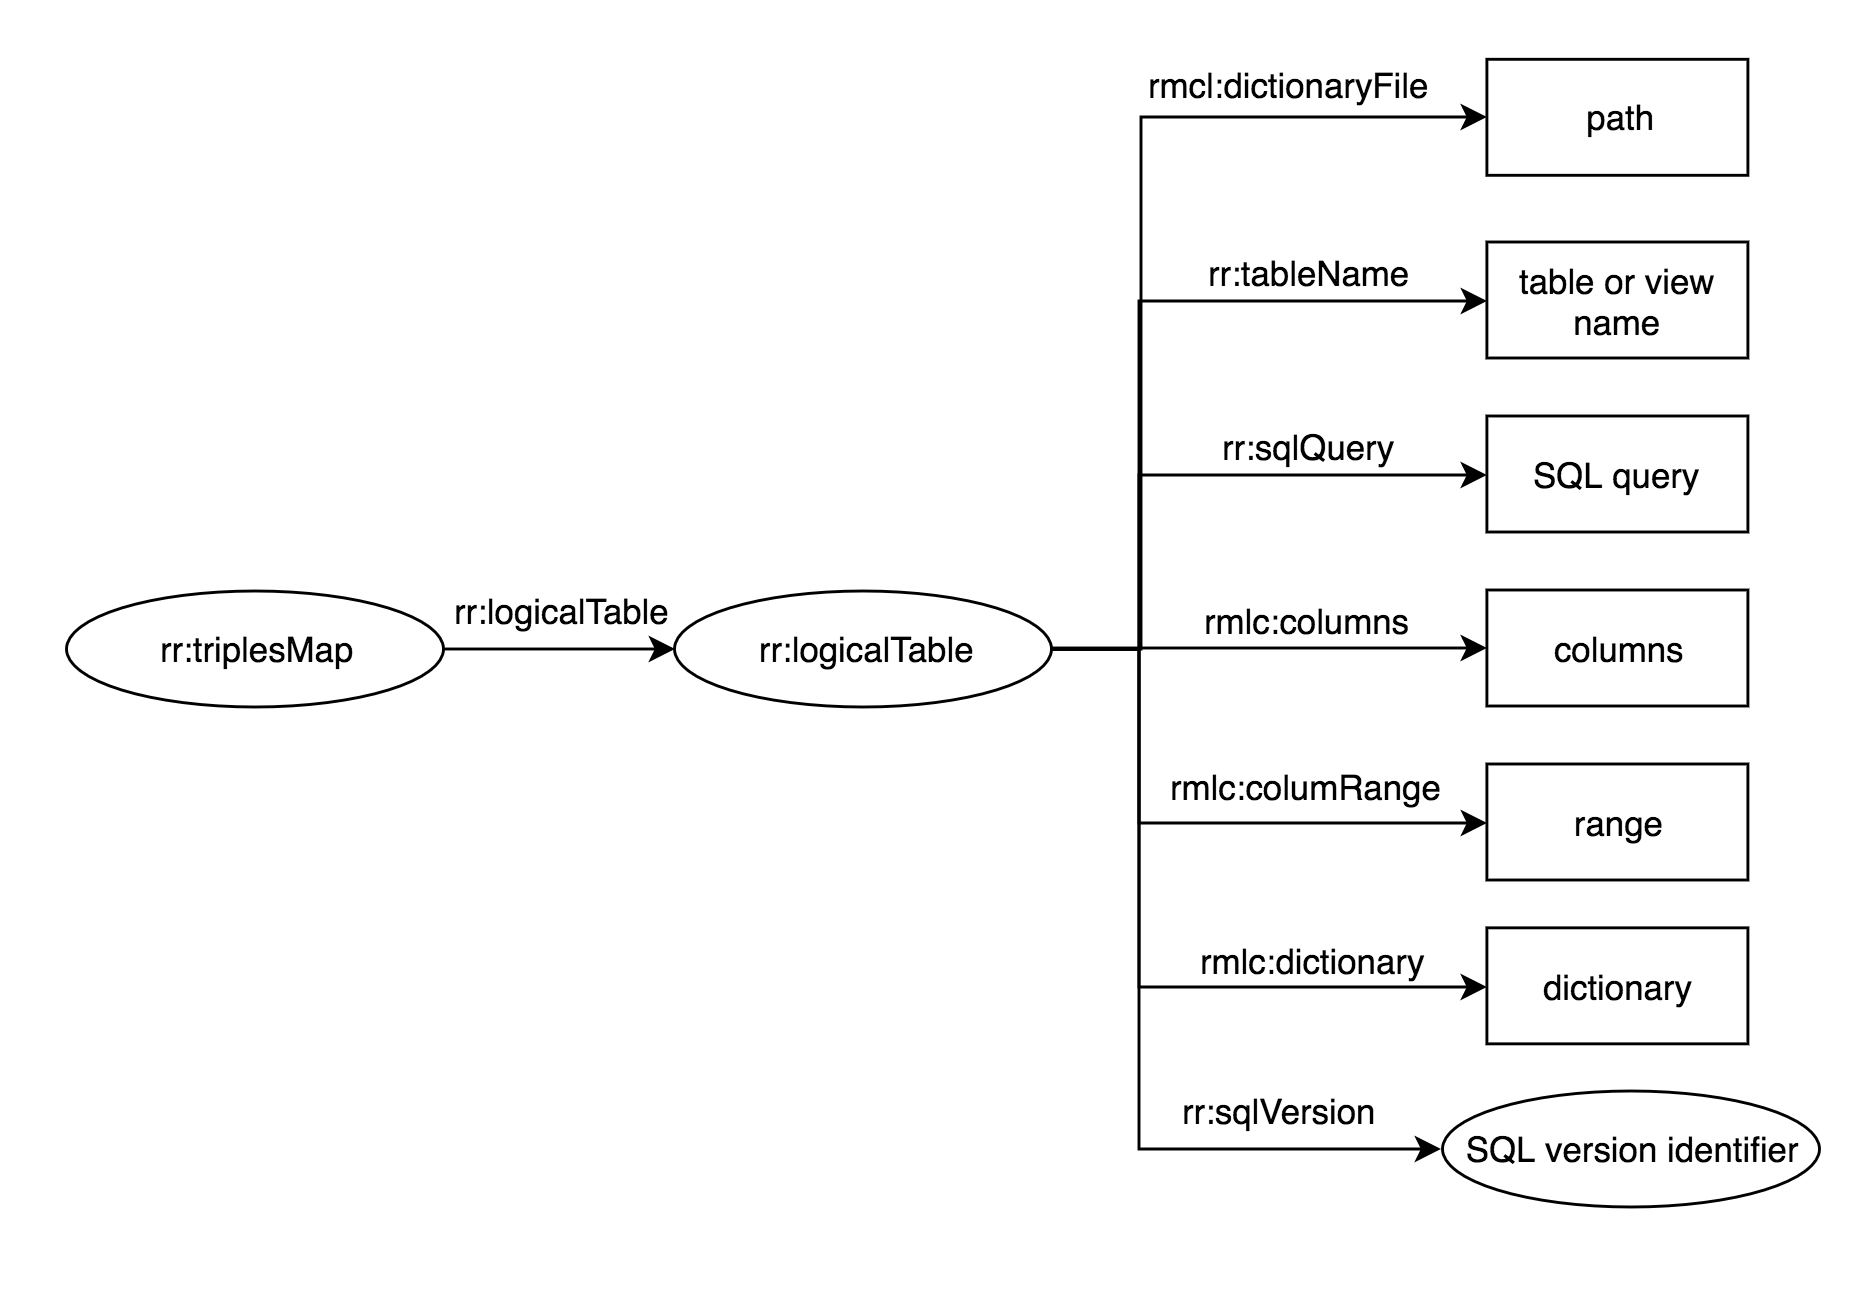
\includegraphics[width=1.0\linewidth]{figures/rmlc-iterator.png}
  \caption{R2RML extension for statistics tabular data}
  \label{fig:rmlc}
\end{figure}
\lstset{upquote=true}
\begin{lstlisting}[float,caption=Columns and dictionary properties in R2RML-Iterator,frame=tlrb,label={list:columns}, columns=fullflexible]
rr:logicalTable [
    rr:tableName "\"2016-P21\"";
    rmlc:columns ("Jan" "Oct" "Dec");
    rmlc:dictionary ("Jan:January" "Oct:October","Dec:December");
];
\end{lstlisting}

\begin{lstlisting}[float,caption=Iterator variables in the extension,frame=tlrb,label={list:iterator}, columns=fullflexible]
<TriplesMap2016{$column}>

rr:subjectMap [
    a rr:Subject;
    rr:template "http://ex.org/2016{$column}";
    rr:termType rr:IRI;
    rr:class qb:Observation;
];
rr:predicateObjectMap[
	rr:predicate sltsv:month;
    rr:objectMap [
    	rr:termType rr:IRI;
        rr:constant "http://reference.data.gov.uk/def/intervals/{$alias}";
    ];
];
rr:predicateObjectMap[
    rr:predicate sltsv:numberOfArrivals;
    rr:objectMap [
        rr:termType rr:Literal;
        rr:column {$alias};
        rr:datatype xsd:integer;
    ];
];
\end{lstlisting}
\lstset{upquote=false}



\begin{table}[t]
\centering
\caption{Excerpt of statistics data to be transformed follow RDF Data Cube data model}
\label{tab:example-stadistics}
\resizebox{\textwidth}{!}{%
\begin{tabular}{l|c|c|c|c|c|c|c|c|c|c|c|c|c}
\hline
\textbf{CountryofResidence} & \textbf{TOTAL} & \textbf{Jan} & \textbf{Feb} & \textbf{Mar} & \textbf{Apr} & \textbf{May} & \textbf{Jun} & \textbf{Jul} & \textbf{Aug} & \textbf{Sep} & \textbf{Oct} & \textbf{Nov} & \textbf{Dec} \\ \hline
Canada      & 44122  & 4016  & 3521  & 3900  & 2962  & 3319 & 4111 & 5330  & 5044  & 2527  & 2345  & 2447  & 4600  \\ \hline
USA         & 54254  & 5144  & 4851  & 5265  & 3408  & 3538 & 3917 & 4919  & 4061  & 3276  & 3432  & 4223  & 8220  \\ \hline
Austria     & 16995  & 2463  & 2917  & 1949  & 774   & 596  & 395  & 1456  & 1232  & 649   & 1063  & 1422  & 2079  \\ \hline
Belgium     & 14387  & 1285  & 1552  & 1639  & 675   & 377  & 586  & 2705  & 1511  & 1180  & 688   & 839   & 1350  \\ \hline
Denmark     & 18097  & 2892  & 3029  & 2216  & 679   & 490  & 1096 & 2632  & 783   & 502   & 921   & 896   & 1961  \\ \hline
France      & 96440  & 9878  & 14602 & 11175 & 7518  & 3281 & 3659 & 10949 & 10805 & 5008  & 5849  & 5845  & 7871  \\ \hline
Netherlands & 41373  & 3194  & 3555  & 2442  & 2496  & 1458 & 1711 & 9755  & 4726  & 2915  & 2272  & 2941  & 3908  \\ \hline
Italy       & 29791  & 4131  & 3607  & 2683  & 1455  & 1010 & 1390 & 2418  & 4517  & 1392  & 1274  & 1803  & 4111  \\ \hline
Norway      & 12790  & 1164  & 1336  & 1318  & 496   & 374  & 1825 & 2260  & 644   & 504   & 808   & 877   & 1184  \\ \hline
Spain       & 19425  & 984   & 1054  & 1587  & 856   & 719  & 735  & 2371  & 3888  & 1846  & 1758  & 1691  & 1936  \\ \hline
Sweden      & 21589  & 3715  & 3277  & 2339  & 771   & 416  & 859  & 937   & 498   & 466   & 1305  & 1943  & 5063  \\ \hline
Switzerland & 26282  & 2483  & 2580  & 2122  & 1870  & 966  & 1208 & 5540  & 1672  & 1432  & 2103  & 1695  & 2611  \\ \hline
UK          & 188159 & 16253 & 19194 & 21430 & 12006 & 8412 & 9406 & 23948 & 20475 & 12288 & 10964 & 13337 & 20446 \\ \hline
\end{tabular}%
}
\end{table}

Listing \ref{list:columns} depicts an example of the usage of the \texttt{rmlc:columns} property, in which the subset of the CSV columns (see Table \ref{tab:example-stadistics}) to be used in the transformation process is specified. This property is defined using a LogicalTable object. We use the \texttt{rmlc:dictionary} (or its corresponding \texttt{rmlc:dictionaryFile}) property to establish a correlation between a column and its alias, that is useful in some parts of the mappings. These properties are based on JSON syntax for easing their creation to the mapping editors.

During the mapping translation process, the variables are replaced with the name of each column or its alias, as defined in the LogicalTable object. The resulting R2RML mapping contains as many TriplesMap objects as the number of columns specified in the R2RML-iterator properties. In this example, the identifier of each TriplesMap, the URI of the subjects and the object of the \texttt{sltsv:numberOfArrivals} predicates, include the variables so they will be replaced with the name of a column or its alias. The R2RML mapping will contain three TriplesMap objects, one for each defined column. All the iterator variables can be specified anywhere in the mapping, as shown in Listing \ref{list:iterator}, using the \{\$column\} or \{\$alias\} syntax.

In order to ensure that the iterator proposal aligns with R2RML, we have developed a mapping translator that converts its mapping document with an iterator variable to a R2RML mapping with multiple TriplesMap objects. In this way, we reduce the size of the R2RML mapping document, minimizing the time of the mapping creation and supporting an easier maintenance. Besides, as it is aligned to R2RML, any R2RML available processor is able to deal with our approach. 

\subsection{R2RML iterator: Use Cases}
In this section we describe our experiment of transforming two statistics datasets from two different domains and agencies: a tourism statistics dataset from the Sri Lanka Tourism Development Authority (SLTDA) and a immigration statistics from the EuroStat. For each dataset, we use both R2RML and R2RML-Iterator mappings with Morph-RDB to generate virtual SKGs and evaluate three SPARQL queries for each one.

\subsubsection{Case 1: Statistics from the Sri Lanka Tourism Development Authority}
\noindent\paragraph{Dataset and Queries.}
The Sri Lanka Tourism Development Authority performs data collection and market research about tourism in Sri Lanka and publishes comprehensive statistics as PDF files\footnote{\url{http://www.sltda.lk/statistics}}. We use tabula-java\footnote{\url{https://github.com/tabulapdf/tabula-java}} to extract these statistics as CSV files and make them available online. For example, the CSV file that contains the number of passengers grouped by countries (y-axis) and the arrival months (x-axis) in 2016.

Our intention is to transform that CSV file into a virtual SKG. Because this SKG is not materialized, there is no need to store it in a dedicated triple store. Any R2RML engine with query translation support will be able to answer SPARQL queries posed to the dataset. For example, consider the following three queries:
\begin{itemize}
\item Q1: Retrieve observations of the number of incoming tourist originated from Spain in 2016.
\item Q2: Retrieve observation of the number of incoming tourists in May 2016.
\item Q3: Can be seen as the combination between Q1 and Q2, i.e., retrieve observations of the number of incoming tourists from Spain in May 2016. 
\end{itemize}

\noindent\paragraph{Mappings.}
The R2RML mapping document generated using the naive approach described in the previous section contains 12 TriplesMaps and around 700 lines. Each TriplesMap describes the transformation rules of the number of arriving passengers every month of the year. Except for those PredicateObjectMap properties corresponding to the name the CSV columns, all TripleMaps have identical values. 

On the contrary, the corresponding proposal mappings, either with \texttt{rmlc:column} property or with \texttt{rmlc:range} property have only 74 lines in total with 1 TriplesMap and 5 PredicateObject mappings. The Table \ref{table:compare1} summarizes the characteristics of the mappings.

\begin{table}[tbp]
\caption[R2RML vs R2RML-iterator in Sri Lanka dataset]{Comparison between R2RML and R2RML-iterator mappings used in the Sri Lanka Tourism dataset example.}
\label{table:compare1}
\begin{tabular}{c|c|c}
\hline
\textbf{Features} & \textbf{R2RML}   & \textbf{R2RML-iterator}  \\ \hline
Total Lines   & $\sim$700 & 74 \\ 
\#TriplesMaps / \#SubjectMaps     & 12                & 1           \\
\#PredicateObjectMaps  & 60              & 5            \\ \hline
\end{tabular}
\end{table}

\subsubsection{Case 2: EuroStat - Immigration Statistics}
\noindent\paragraph{Dataset and Queries.} Eurostat\footnote{\url{http://ec.europa.eu/eurostat}} publishes the statistics office of the European Union. Its main responsibility is to provide statistics information about European Union such as economy, finance, population, industry, etc. In this example, we consider a dataset containing the number of immigrants that have arrived in European countries available online\footnote{\url{http://ec.europa.eu/eurostat/product?code=tps00176&mode=view}}. We downloaded the aforementioned dataset as a CSV file containing the number of immigrants grouped by countries (x-asis) and years (y-axis). We have created three SPARQL queries, similar to the ones in the previous example:

\begin{itemize}
\item Q1: Retrieve the number of immigrants arriving in Spain.
\item Q2: Retrieve the number of immigrants arriving in any of European Countries in the year of 2015.
\item Q3: Retrieve the number of immigrants arriving in Spain in the year of 2015.
\end{itemize}

\noindent\paragraph{Mappings.}
Generating the naive mapping described in the first approach is not feasible in this case, as there is a need to generate a TriplesMap for each column that represents a country and the dataset contains more than 40 columns. Instead, we generate two R2RML-iterator mapping documents,one with \texttt{rmlc:columns} property and the other with \texttt{rmlc:range} property. Then we use the our mapping translator engine to generate the naive version of R2RML.

Our proposals mapping document (either version) contains only 1 TriplesMap and 4 PredicateObjectMap mappings, totalling less than 70 lines. On the contrary, the generated R2RML mapping document has more than 40 TriplesMap, more than 170 PredicateObjectMap mappings, totalling more than 2800 lines. The Table \ref{table:compare2} summarizes the characteristics of the mappings.
\begin{table}[tbp]
\caption[R2RML vs R2RML-iterator in Eurostat dataset]{Comparison between R2RML and R2RML-iterator mappings used in the Eurostat Immigration dataset example.}
\label{table:compare2}
\begin{tabular}{c|c|c}
\hline
\textbf{Features} & \textbf{R2RML}   & \textbf{R2RML-iterator}  \\ \hline
Total Lines   & $>$2800 & $<$70 \\ 
\#TriplesMaps / \#SubjectMaps     & $>$40                & 1           \\
\#PredicateObjectMaps  & $>$170              & 4            \\ \hline
\end{tabular}
\end{table}


\section{Conclusions}

In this chapter, we have discussed the concept of mapping translation, which had not been addressed before in the literature. We have shown how this concept has been actually implemented in some approaches addressing the readability and maintenance of mappings, the generation of programming code to provide access to heterogeneous data sources, or the enrichment of original data sources, among others. Additional, the mapping translation concept is the main idea behind the optimizations proposed in this thesis and described in detail in Chapter \ref{chapter:virtual} and Chapter \ref{chapter:construction}.

We think that this concept needs to be explored further, and this would allow a new range of KGC approaches that may be part of a new generation, as claimed in the title of the chapter. The KGC community\footnote{\url{https://www.w3.org/community/kg-construct/}} should see this variety of mapping languages not only as challenges (e.g., interoperability) but also, and mainly, as an opportunity for further research and development in this area, to address the need to cover more types of data sources while taking advantage of all the work that has been done in advanced aspects like query translation. Providing mapping translator services across mapping languages would bring further benefits and increase the availability of ontology-based data for its exploitation by search engines and query answering systems at Web scale.